\chapter{绪论}
\section{研究背景及研究意义}

\subsection{研究背景}
通信的主要目的是传递信息。 
无论是在传统的有线通信系统还是在无线通信系统中,由于信道传输特性的限制,
基带信号不能直接通过信道传输,而是需要对基带信号进行调制以将其搬移到 一定的频段进行有效地传输\cite{昌信2006通信原理}。 
同时,对基带信号的调制,还可以使通信系统在具有更高的传输速率的同时,提高频谱利用率。\par

随着通信技术的不断发展,终端的数目呈爆发性增长,用户对信息传输速率和传输稳定性的要求不断提高。
为了满足这样的需求,通信信号的调制形式由简单到复杂,调制方式由传统的模拟调制发展到主流的数字调制方式,
信道从有线信道到有线与无线信道混合组网。
调制是指将发送的信号加载到高频(基带调制除外)信号以适应信道传播环境的一种技术。
调制方式自动识别,是指在未给定调制信号所携信息的情况下,利用学习的算法,
通过接收信号电磁特性判定信号的调制方式。
模拟调制针对的是模拟信号,传统的模拟调制按照调制方式的不同,
可以分为幅度调制(AM)、频率调制(FM)和相位调制(PM)等;
数字调制针对的是数字信号,按照调制方式的不同可以分为
幅移键控(ASK)、频移键控(FSK)、相移键控(PSK)和正交幅度调制(QAM)等。 \par

调制信号的自动识别,是一种优化频谱利用效率,识别和最小化干扰,以及有效推动认知无线网发展的重要手段,
在协作通信和非协作通信中都得到了广泛应用\cite{nandi1995automatic}。
在军事领域,调制识别被广泛地用作通信侦察,电子战和威胁分析,是一种智能信号分析和处理的关键技术\cite{程汉文2009基于累计量的干扰信号调制识别算法}\cite{张春磊2013认知电子战初探}。
在侦听接收机的设计中,获取无线接收信号的调制方式是侦听接收机的重要功能之一。
有效的无线信号调制方式识别为解调器正确选择解调算法提供了参数依据,可以使我们最终得到准确的情报信息。
调制识别技术也有助于为电子战选择最佳的干扰模式或干扰消除算法,以保证我方设备之间通信的稳定性;
同时抑制和干扰对方的通信以达到电子战通信对抗的目的。\par

因此,通信信号调制自动识别技术具有非常广阔的应用前景,将成为未来的民用无线通信以及军事通信中的重要组成部分。\par

深度学习(Deep Learning,DL),是一种机器学习(Machine Learning,ML)领域的分支。
2006年Hinton等人提出了深度置信网络(Deep Belief Network, DBN)\cite{hinton2006fast},并引入了分层预训练技术,自此深度学习得到了广泛的应用。
在目标检测、语音识别、机器翻译等许多不同的人工智能任务中,深度学习已经极大地提升了这些任务上的最佳表现水平\cite{lecun2015deep}。 \par

2012年的ILSVRC2012竞赛中,Krizhevsky等人引入了Dropout等方法,训练了一个大型的深度卷积神经网络AlexNet,
使用深度学习模型击败了Google团队并取得了该竞赛的冠军,
使得图片识别错误率下降了$14\%$\cite{krizhevsky2012imagenet}。
2014年Christian Szegedy等人提出GoogLeNet,打破了常规的卷积层串联的模式,
将$1 \times 1, 3 \times 3, 5 \times 5$的卷积层和$3 \times 3$的池化层并联组合到一起,
以较大优势取得ILSVRC2014冠军并使top-5的错误率降到了$6.67\%$\cite{Szegedy_2015_CVPR}。
2015年,KaimingHe等人设计了一个多达152层的ResNet架构,
使图片识别的错误率也降到了$3.6\%$\cite{he2016deep}。
研究者在将深度学习应用到目标检测、面部识别或语言模型等传统任务的同时,
也在将其扩展到许多不同的现代领域和任务中,
比如Osako等人使用循环神经网络来给语音信号降噪\cite{osako2015complex},
Gupta等人使用堆栈自编码器(stacked autoencoders)来发现基因表达的聚类模式\cite{gupta2015learning},
Gatys等人使用一种神经模型来生成不同风格的图像\cite{gatys2015neural}等等。
深度学习在很多领域都取得了较大的发展。\par

\subsection{研究意义}

在无线通信中,调制识别是正确实现无线通信解调和保证正常接收的重要组成部分。
基带信号通常是频率非常低且分量很多的频谱,这些含有很多低频分量的信号不适合在信道中直接传输,
这就需要我们对基带信号进行调制,以适应信道的特性并在无线信道中进行有效传输。
信号在经过调制并通过信道到达接收端,与原始的信号具有很大的不同。
所以,只有在接收端确定信号的调制方式,才能利用相应的解调方法解调获取原始信息。
基于深度学习的调制识别的意义主要体现在以下几方面:\par

(1) 提高通信设备的稳定性与通用性,降低建设与运维成本。
通信技术的迅速发展导致了各种通信系统的共存,而这些通信系统的调制方式可能各不相同。
由于解调需要与调制进行匹配才能准确地接收发射信号,这些差异性的调制技术也导致接收机类型大幅增加。
于是,人们希望能够通过发展新的无线认知技术,基于通用的接收机平台来接收并识别不同的调制信号,
以减少接收机类型的快速增长。 \par

(2) 军事领域的电子对抗、电磁干扰与反干扰的基础。
当检测到对方无线电信号或电磁信号时,
需要我们对检测到的信号或电磁信息,进行调制识别以及载波频率与波特率等参数的正确估计,
方便接下来的情报获取或者进行电磁干扰。\par

(3) 有助于如何在频域、时域和空域等多维度上有效分配频谱资源,提高频谱利用率。
在认知无线领域,无线频谱资源根据具体业务的不同,
主要划分为民用的广播电视、无线通信、卫星通信及军用的雷达与军事通信等不同频段。
为了避免相邻频段或频道的互相干扰,不同的通信业务的工作频段相互隔离,
并且不同频段之间预留一定的间隔频带;
上下频段的频谱资源分配以及频谱利用率极不平衡,造成了频谱资源的极大浪费。
由于无线频谱资源有限,随着频谱资源的消耗殆尽,
现有的频谱分配与管理机制已经成为制约无线通信进一步发展的重要因素。\par

(4) 利用深度学习的方法提升传统调制识别算法的性能上限。
在通信系统中使用DL有很多优点。 首先,由于通信基础设备以及终端的数量多,且通信数据速率高,因此可以很容易获取DL训练所需要的大量数据。
其次,DL可以自主提取特征,避免了手动特征选择这一繁琐且具有挑战性的任务。
另外,新的、更复杂的信号和通信应用的出现,给认知无线带来了更大的挑战;
有时,我们需要对一些未知的信号进行认知,而传统的基于特征的方法在新的场景下很难适应信号特性的变化。
因此,我们可以利用深度学习的特征自提取能力,来增强对于未知信号的认知能力。\par

(5) 促进深度学习在通信领域的发展。
在调制识别领域中,利用专家特征和判决准则进行调制识别得到了广泛的应用,
并且在特定情况下可以实现很高的识别准确率。
深度学习在计算机视觉和自然语言处理等领域的应用,绝大多数是基于数据进行特征与模型的学习,
而不是利用专家知识提取特征进而训练模型,这与很多传统的机器学习算法(比如DNN、支持向量机、决策树等)在算法思想上有很大不同。
而且,这些基于数据的深度学习算法在相应的领域取得了最好的性能。
因此,这就需要我们重新审视一下,是否也应该对通信领域的传统算法在思想上进行改变,
基于数据去理解信号,去学习信号本身的特征。\par

\section{无线信号调制识别的发展和研究现状}

早期调制识别的任务是由操作人员在仪器的帮助下完成的:
主要是通过观察和分析接收信号的时域波形和频谱形状,判断信号的调制方式,然后选择相应的解调器进行解调。
然而,随着无线通信技术尤其是数字通信技术的快速发展,信号调制方式变得越来越复杂,很难通过人工的方法来准确判别调制方式的类别。 
C.S.Waver等人于1969年在斯坦福大学发表了第一篇关于通信信号调制识别的论文\cite{weaver1969automatic},
此后,调制方式的自动识别引起了人们的广泛关注,各种技术出版物上出现了许多关于调制识别的文章,
其中许多结果已经被应用到实际工作中。 \par

对于无线信号调制识别的研究,现有算法大致可以分为:基于假设检验的最大似然法,
基于特征提取的模式识别方法,以及基于深度学习的调制识别方法。
大多数基于假设检验的最大似然类方法计算复杂度较高,对模型失配问题较为敏感,这大大限制了它们在实际通信环境中的应用。
基于特征提取的模式识别方法,通常关注能量在不同频段上的分布,并使用专家特征和判别准则来识别和区分特定的调制方式。
在特定的条件下,基于特征的方法可以实现接近理论最佳的识别性能,并且其具备较强的鲁棒性,
因此得到更广泛的应用。
鉴于深度学习在其他领域取得的成果,深度学习可以与硬件结合自适地进行学习提高传统算法的性能上限,
并可以通过特定的正则化方法来降低过拟合提高模型的鲁棒性。
因此,深度学习在通信领域近年来已经成为一个研究热点,在调制识别领域也有很多人投入到相应的研究中。\par

\subsection{基于似然比判决理论的方法}

基于似然比决策理论的方法也叫做最大似然假设检验法。 
其基本思想是使用概率论和假设检验理论来分析信号的统计特性,
并依据损失函数最小化原则获取足够的统计信息,定义判决准则,对信号进行分类。
基于似然比判决理论的调制识别系统框图如图\ref{sec:fig_1_0}所示。\par

\begin{figure}
	\centering
	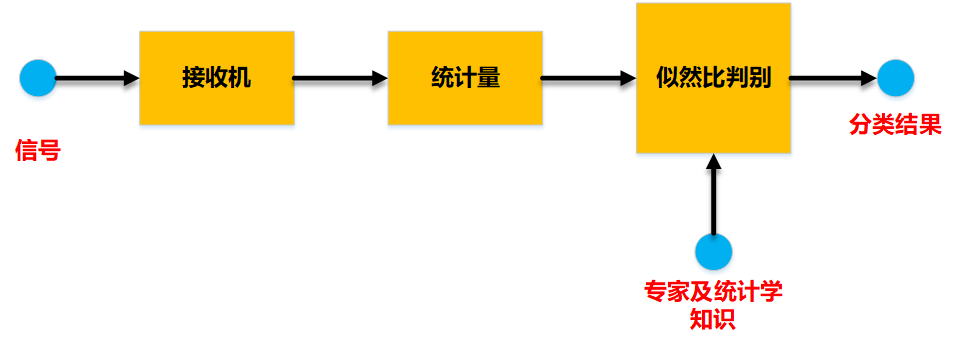
\includegraphics[scale=0.55]{figures/chapter_1/fig_1_0}
	\caption{基于似然比判决理论的调制识别系统框图} \label{sec:fig_1_0}
\end{figure}

对于现有调制识别的发展,Kim和Polydoros\cite{kim1988digital}使用平均似然比检验来识别BPSK和QPSK信号。
Hwang等人通过似然方法法解决了数字正交偏移调制信号的分类问题\cite{hwang1991advanced},
Chung-Yu Huan等人针对加性高斯白噪声中对MPSK调制进行分类的问题,
提出了基于似然函数及其近似的算法\cite{380199}。
Schreyoegg等人提出了一种分类QAM信号的星座图方法,
主要通过分析幅度分布和相位直方图的DFT来对多种QAM信号进行区分\cite{644992}。 
Wei和Mendel将最大似然方法应用于数字正交调制的分类,并分析了最大似然分类器的渐近行为,
当信噪比为5dB时,准确率接近$100%$\cite{wei2000maximum}。
Boiteau等人提出了一种广义的似然比调制识别框架,作者首先对似然比函数中自然指数进行幂级数展开,
然后对未知参数做期望平均处理,实质上应用了高阶统计量\cite{boiteau1998general}。
\par

基于似然比决策理论的算法的优势是:在理论上保证贝叶斯最小误判准则,使分类结果最优;
同时,它可以通过理论分析得到分类性能曲线。
但是他同时具有很多局限性:
首先,现有的似然比决策理论算法主要处理符号的同步采样序列,他们需要比模式识别方法更多的先验知识,
这意味着我们需要预先知道信号的载波频率,符号速率和符号时序等先验信息;
其次,基于未知参数似然比的分类,需要计算复杂的统计表达式,计算成本较高,很难对信号进行实时处理;
第三,基于似然比决策的算法对模型失配和参数偏差较为敏感,即鲁棒性较差。
基于似然比函数的分类,通常将参数值建模为高斯分布,并且需体现知道信噪比等参数。
当实际信道噪声为非高斯噪声时,或者存在多径影响、多信号干扰以及SNR参数估计偏差较大时,
分类的性能可能会急剧下降。\par
 
\subsection{基于特征提取的统计机器学习方法}

基于统计机器学习的调制识别系统大都具有相同的范式:
首先从信号中提取先前选择的特征,然后利用训练好的机器学习模型进行调制识别。
它主要包括特征提取子系统和机器学习子系统,其整体系统框架如图\ref{sec:fig_1_1}所示。\par

\begin{figure}
	\centering
	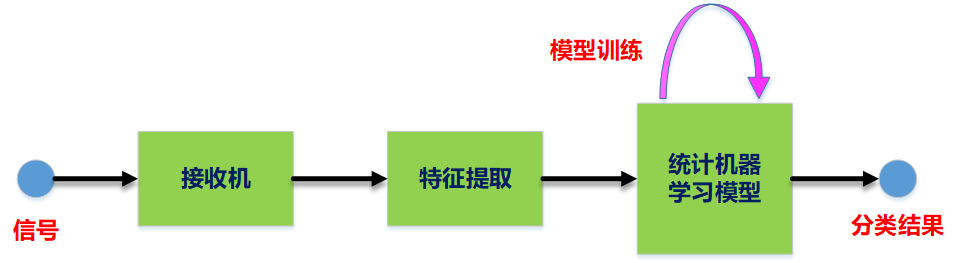
\includegraphics[scale=0.6]{figures/chapter_1/fig_1_1}
	\caption{基于统计机器学习的调制识别系统框图} \label{sec:fig_1_1}
\end{figure}

特征提取子系统主要从未处理信号中提取所需的特征分量,如瞬时频率,瞬时相位和瞬时幅度等。 
模式识别子系统的主要功能是通过特征子系统提取的特征分量对模型进行训练;
模型训练好以后,当需要判别的信号进入该子系统,我们的模型可以对不同的调制信号进行分类。\par

Liedtke提出了一种用于未知调制方法分类的通用分类器,
对数字调制信号识别方法首先进行公开讨论\cite{liedtke1984computer}。 
该算法主要对幅移键控(ASK),具有小频偏的频移键控(FSK)和相移键控(PSK)等信号进行了识别,对于噪声、频率偏移、带宽不匹配以及邻域信号串扰等影响,具有较强的可靠性和鲁棒性。 
Azzouz等人提出了一套用于识别不同类型数字调制方式的判别标准,
它使用相位的非线性部分及其绝对值,归一化的瞬时振幅和频率等特征,
在信噪比SNR = 10dB时,调制类型分类正确率大于$90\%$\cite{azzouz1995automatic}。
M.L.D. Wong和AK Nandi等人提出了利用多层感知机进行调制识别的算法,
该算法具有更好的泛化能力,并增加了一个新的基于统计累积量的特征集来识别十种不同的调制类型;
即使在低信噪比条件下,该算法也具备较好的性能,
在SNR=0dB时,识别准确率可以达到$98\%$\cite{wong2001automatic}。
汤卫东利用小波变化对调制信号进行了类内和类间识别,提高了低信噪比条件下的识别率\cite{汤卫东2010基于小波变换的数字通信信号调制识别研究}。
杨发权在其博士论文中,对高维数据块正交调制识别方法进行应用,并对MLP在调制识别中的应用进行了研究,
实现了在低信噪比条件下基于星座图的调制识别\cite{杨发权2015无线通信信号调制识别关键技术与理论研究}。\par

高阶统计量是描述随机过程的高阶统计特性的数学工具,包括高阶矩和高阶累积量,以及高阶周期矩和循环累积量。
Reichert和Juergen首次提出使用高阶统计量来识别2ASK,2PSK, 4PSK,2FSK,MSK等信号,
之后基于高阶统计量的调制信号识别方法取得了很大进展\cite{reichert1992automatic}。
Swami提出了一种基于四阶累积量的数字调制识别的算法,对2ASK,2PSK,4PSK,MSK和2FSK的信号进行识别,
当信噪比为7.3dB以下时,识别率都能超过$97.9\%$\cite{swami2000hierarchical}。
Gardner和Spooner第一次将循环谱域的结构可分性应用到信号分类,
之后KIM等人利用循环谱特性构建分类器来识别SQPSK和$2^k$PSK信号。\par

基于星座的调制识别将调制识别问题转化为形状识别问题。
Mobasseri首先提出了星座图作为调制识别的一种强特征,
利用二项非均匀空间随机场恢复星座图,并利用机器学习算法作为分类器,
在高噪声环境中具备较强的稳定性\cite{mobasseri1999constellation}。
接下来,Mobasseri又证明模糊C均值聚类能够恢复未知星座,使用星座形状作为数字调制识别的强特征,
通过ML规则对未知星座形状的信号进行分类,
该算法适用于任意大小和维度的数字调制\cite{mobasseri2000digital}。\par
 
对于以上提到的各种分类特征,包括时频统计特征,高阶统计量,星座特征等,
大部分是针对特定类型信号的,而不是对所有的信号都具备一定的辨识能力。
另外,大多数现有的调制识别算法都假定信道是理想的高斯白噪声信道,并且只有少数算法研究了衰落信道。
在实际应用中,无线信道的衰落现象不容忽视,多径效应使得传输信号间存在码间干扰等。
在基于理想高斯白噪声信道环境的识别算法中,信噪比较高时识别性能较好;
当信噪比较低时,算法估计的瞬时包络,相位和频率参数可能会存在较大的误差,使系统的识别性能急剧下降,
并且稳定性差,不能满足实际应用的需求。\par

\subsection{基于深度学习的无线调制识别方法}

深度学习是机器学习中一种基于对数据进行表征学习的方法。
深层神经网络是由一系列层组成网络,其中每一层通常是由已知的具有可调参数和非线性激活函数的线性单元组成,
使得深度网络最后可以拟合高度非线性的函数。\par
深度学习在通信领域的应用,带来了新的机遇与变革。
O'Shea等人第一次将卷积神经网络(Convolutional Neural Network, CNN)引入调制识别,证明了深度学习可以应用在调制识别领域,
并且在低信噪比条件下具有更加稳定的性能\cite{o2016convolutional};
此外,作者还提供了一个用于调制识别学习的基准数据集\cite{o2016radio}。
Mendis等人将深度置信网络(Deep Belief Networks, DBN)引入到调制识别,
在多径信道下,信噪比在$0dB$以上时检测准确率达到$90\%$以上,分类准确率达到$85\%$以上\cite{mendis2016deep}。
Afan等人提出了一种基于非负约束自编码器的自动调制分类的方法\cite{ali2017automatic}。
相较于传统的稀疏编码,该方法提高了稀疏性并使重构误差最小,在有限的信号长度和衰落信道条件下具有较高的准确率。
Rajendran等人提出了一个基于长短期记忆网络(Long Short-Term Memory,LSTM)的调制识别网络,
在信号的信噪比从0dB到20dB的不同SNR条件下,
平均分类准确率为90%左右\cite{rajendran2017distributed}。
Bin Tang提出了一种基于生成对抗网络(Generative Adversarial Net-works,GAN)增强的通信信号调制分类算法,
弥补数据不足对网络训练的影响,作者提出增强数据的方法,
使模型的分类精度可以提高0.1\% ~ 6.0\% \cite{8319926}。\par

以上的研究主要是从应用的层面对深度学习的既有方法进行不同领域的迁移应用,
并没有提出一定的算法框架或者底层网络结构的改进,而且对于影响性能的因素,算法所能达到的上限,
以及将深度学习与传统的调制识别方法结合方面都没有进行相应的研究。
因此,需要我们对深度学习在调制识别中的应用在算法、框架、应用等层面进行更深入的研究,
以提高系统的调制识别性能。\par

\section{本文主要工作及内容安排}
从现有的研究成果可以看出,虽然数字通信信号的调制识别算法有很多,
但能够直接利用原始数据对调制信号进行识别的算法还比较少,大多都需要手动进行专家特征提取,
进而训练机器学习模型进行调制识别。
而在实际的非协作通信中,受环境的影响,我们学习的模型在不同的环境中分类性能差别很大,鲁棒性较差。
现有的基于深度学习的调制识别算法,并没有对影响网络性能的因素进行分析,也没能有效利用过去几十年的研究成果。\par

本文提出了一种基于卷积自编码器和卷积神经网络框架
(Convolutional Autoencoder - Convolutional Neural Network,CAE-CNN)的调制识别算法,
并提出了相应框架下的网络训练方法;
提出了一种将深度特征与传统特征进行融合的算法框架,并对特征融合的方式进行了研究;
研究了网络的深度、网络底层模块结构等对调制识别性能的影响,分析了不同情况下造成网络识别性能变化的因素。 \par

本文的具体内容安排如下:

第一章为绪论。首先对无线信号调制识别技术的研究背景进行了介绍,
系统的阐述了现有的调制识别的算法,并对当前的研究现状进行了总结概括。\par

第二章首先介绍了调制信号的基本概念,然后分析了信道对于调制识别的影响;接下来,介绍
了神经元、前馈神经网络、卷积神经网络、自编码器等深度学习的基本
理论和基本网络架构;最后,介绍了最近较为流行的几种神经网络优化算法,并分析
了各种算法的一些理论基础。 \par

第三章提出了一种CAE-CNN调制识别的算法框架,并提出了相应的训练算法。
我们分别利用监督方法和无监督方法将信号特征可视化,
利用无监督的卷积自编码器可以复现输入信号,并获得原始信号的低维表示;
通过有监督的CNN获取的信号低维表示,得到对于不同类别具有区分度的特征;
利用t-分布随机邻接嵌入(t-distributed stochastic neighbor embedding,t-SNE)算法,
将信号的低维表示降到二维的流型中,观察了信号的分布状况。
我们融合卷积自编码器与卷积神经网络,提出了一种CAE-CNN算法框架和相应训练算法。\par

第四章提出了一种传统特征与深度特征融合的框架。
首先概括了传统调制所用到的调制识别特征,然后阐述了体征融合的基本理论。
接下来,将传统方法中常用的调制识别的特征与CNN获取的深度特征进行适应性的$Batch-Normalization$,
分别针对Softmax、随机森林、深度神经网络等融合算法构建融合模型,
并对不同的融合算法进行了仿真。 \par

第五章从网络底层研究网络超参数对调制识别性能的影响,并从欠拟合
与过拟合以及偏差与方差的角度来理解出现这些现象的原因。
首先,构建了调制识别模型的偏差与方差模型,并阐述了过拟合与欠拟合的原因;
然后,基于CNN网路框架研究了卷积核数目、大小以及卷基层深度对调制识别的影响。\par

第六章对本文的工作进行了总结,从深度框架、特征融合、网络超参数等三个点阐述了
本文所做出的贡献。同时,对深度学习在调制识别领域的应用进行了展望,对以后打算开展的
研究做了一定的概述。
\par